%======================================================================
\section{Data assimilation in the local latent field}
\label{sec:da_results}
%======================================================================

Part~II asks whether the local structure that lets a model transfer
also lets a filter work on large domains with a fixed ensemble. The
models are those of Part~I, deployed at each size without retraining;
the filters run entirely in their latent space and observe the physical
field.

%----------------------------------------------------------------------
\subsection{Setting: exact locality and what is measured}
\label{sec:da_setting}
%----------------------------------------------------------------------

\para{Twin experiments.} At each domain size the truth is a trajectory of
the PDE itself, integrated at the deployment resolution from a spun-up
state. Every $5$ model steps (5 time units in 1D, $0.5$ in 2D KS, about
$0.5$ and $0.1$ Lyapunov times) we observe the field at the points of a
regular network with spacing $3.125$ (1D) or $2.75$ (2D KS) length
units, two observations per site in 1D and four in 2D, with independent
Gaussian errors of standard deviation $0.1$ in the standardized units of
the training data. The initial ensemble is the encoded initial truth
plus independent perturbations of standard deviation $0.1$ per latent
coordinate; the forecast adds model noise of standard deviation $0.08$
per coordinate at every step (Sec.~\ref{sec:da_method}). Each run has
$100$ cycles. The free run starts from the same ensemble, evolves with
the same model, receives no observations and no model noise; the error
of its ensemble mean is the reference that skill is measured against.

\para{Filters.} Section~\ref{sec:da_method} defines the three analysis
schemes. We name them by what they compute, since the literature uses
``LETKF'' for several. The \emph{dense filter} is a stochastic ensemble
Kalman filter (EnKF) with perturbed observations and Schur-product
localization of the full $\dlat\times\dlat$ forecast covariance. The
\emph{per-site filter} performs one analysis per site, in the
local-analysis form of \citet{hunt2007}, with each observation's error
variance divided by its taper value, but with the same
perturbed-observation update as the dense filter; it is therefore a
local stochastic ensemble Kalman filter rather than an ensemble
transform filter. Its deterministic counterpart, the local ensemble
transform Kalman filter of \citet{hunt2007} with the same localization,
gives the same skill to within $2\%$ at $\Nens=64$ (Appendix~\ref{app:da}) and is
reported where it differs. In 1D the analysis is also done with the
particle flow filter (PFF), and both 1D filters use the same Gaspari--Cohn
(GC) taper of half-width $3$ sites.

\para{Why the per-site filter is exact.} The decoder of the 2D models is
per-patch ($\Rdec=0$), so by Proposition~\ref{prop:blockdiag} the
Jacobian of the observations with respect to the latent field is
block-diagonal: an observation depends only on the $c$ channels of the
site whose patch contains it. Two consequences make the filter scale.
The whole Jacobian is obtained from $c=6$ forward-mode derivatives at
any domain size, and each site's analysis uses only the ensemble at the
few sites that own an observation inside its taper support, without
truncating any observation's dependence on the latent state. The local
analysis is not an approximation of a global one that happens to be
local; it is the analysis of a problem that is local. The dense filter,
by contrast, stores $\dlat\times\dlat$ matrices, whose memory grows with
the square of the area.

\para{Metrics.} The \emph{error} at an analysis time is the
root-mean-square difference, per latent coordinate, between the
ensemble-mean latent field and the encoded truth,
$\|\bar z - \E(u)\|/\sqrt{\dlat}$; the free run's error is defined the
same way. \emph{Skill} is the ratio of free-run error to analysis error:
above 1 the filter helps, below 1 it makes the estimate worse than not
assimilating at all. \emph{Spread} is the ensemble standard deviation per
coordinate, and \emph{calibration} the ratio of spread to error, which is
1 for an ensemble that represents its own uncertainty correctly and
below 1 for an over-confident one. All reported values are
\emph{steady-state} averages over cycles $51$--$100$, after the initial
transient. Because the latent coordinates are learned, we also measure
the error in physical space: the root-mean-square difference between
the decoded ensemble mean and the true field, at every grid point and at
the observed points separately, against the floor set by the decoder
alone, $\|\Dec(\E(u))-u\|$.

\para{How large an ensemble the problem demands.} Without localization a
filter needs at least as many members as there are unstable and neutral
directions \citep{bocquetcarrassi2017}; for a deterministic filter on
Lorenz-96 the minimum is $n_+ + 1$, with $n_+$ the number of positive
Lyapunov exponents \citep{takeda2026}. These counts are measured here.
For 2D KS the truth has $n_+ = 42$--$44$ at $44^2$ and $93$--$101$ at $66^2$,
and the transferred model has $n_+ = 168$--$170$ at $88^2$ (Table~\ref{tab:truth}
and Appendix~\ref{app:tables}); for 1D KS the truth has $n_+ = 26$--$27$ at
$L=200$ and $50$--$51$ at $L=400$ (Appendix~\ref{app:truth_list}). A fixed ensemble of 64 members is therefore above
this bound only at the native 2D size and at $L=200$ in 1D. An
unlocalized filter of that size should fail beyond them; a localized
filter needs only to span the unstable directions inside its taper
support, Eq.~\eqref{eq:nens_local}, which do not grow with the domain.
The following sections test both predictions.

%----------------------------------------------------------------------
\subsection{A fixed ensemble across a hundredfold area}
\label{sec:da_2d}
%----------------------------------------------------------------------

Table~\ref{tab:da_2d_sizes} and Fig.~\ref{fig:da_2d} give the central result of Part~II. The 2D KS
model, trained on windows of a $264^2$ simulation, is deployed on square
domains from $44^2$ to $440^2$, a factor of 100 in area and in latent
dimension ($\dlat=384$ to $38\,400$), and the same per-site filter with 64
members assimilates the same observation network at every size. Its
steady-state skill is $4.23$ at $44^2$ and $3.84$--$4.08$ at every larger size,
$3.90$ at $440^2$: the filter loses less than $10\%$ of its skill over the
whole range. A second seed at every size from $44^2$ to $330^2$ changes the
skill by at most $0.15$.

An unlocalized filter with the same 64 members does what the bound of
Sec.~\ref{sec:da_setting} predicts. At $44^2$, where $64$ exceeds the
$42$--$44$ unstable directions, it helps (skill $2.31$); at $66^2$, with
$93$--$101$, and at $88^2$, with about 170, it is worse than no
assimilation ($0.94$ and $0.83$). Doubling the ensemble to 128 restores
skill where 128 exceeds $n_+$ ($3.47$ at $44^2$, $2.22$ at $66^2$) and not where
it does not ($1.11$ at $88^2$). The dense filter with Gaspari--Cohn
localization, which applies the same taper to the full covariance,
works at every size it can be run at ($3.40$--$3.65$), $11$--$14\%$ below the
per-site filter, but its memory grows with the square of the area
(Sec.~\ref{sec:da_cost}), and beyond $220^2$ we did not run it.

\para{Ensemble size.} Table~\ref{tab:da_2d_ensemble} shows the per-site
filter's skill against ensemble size. It is the same at every domain
size: about $1.1$ with 8 members, $1.8$--$2.1$ with 16, $3.3$--$3.8$ with 32,
$3.8$--$4.2$ with 64 and slightly lower again with 128. That the required
ensemble does not depend on the domain size is the point. The level it
settles at is set by the local problem: Eq.~\eqref{eq:nens_local} with
the 2D KS density of $0.043$ per unit area and the taper's support (radius
$33$ length units) gives an estimate of about 150, far above the 32--64
members that suffice, so the heuristic is conservative here, as one
expects when the errors inside the support are dominated by a few
unstable directions. The dense filter with localization already reaches
$3.5$--$3.8$ with 16 members, where the per-site filter does not. The
deterministic transform behaves like the perturbed-observation update
at every ensemble size ($1.87$ at 16 members), so observation sampling
noise is not the cause. The likely cause is the localization form: the
dense filter tapers the covariance itself, while the per-site filter
tapers only the observation errors and uses the untapered sample
covariance among the sites inside its support, which 16 members estimate
poorly. We have not tested this.

\para{Calibration and model noise.} The ensemble is over-confident:
its spread is about a third of its error at every size ($0.33$--$0.37$ for
the per-site filter, $0.40$--$0.43$ for the dense one). Inflating the
forecast perturbations by up to $20\%$ changes neither skill nor
calibration by more than $9\%$ (Appendix~\ref{app:da}): with four observations per
site, the analysis is set by the observations rather than by the prior
spread. The model noise is the effective control. Halving it from $0.08$ to
$0.04$ raises the skill by $13$--$14\%$ and lowers the calibration by $0.03$, by
the same amounts at $44^2$, $88^2$ and $220^2$ (skill $4.79$, $4.55$, $4.33$), so this
trade-off, too, does not depend on the domain size.

\para{In physical space.} The latent error is measured against the
encoded truth, so it cannot see what the decoder loses. Decoding the
analysis mean, its root-mean-square error against the true field in
steady state is $1.05$, $0.99$, $1.01$ and $1.02$ at $44^2$, $88^2$, $220^2$ and
$330^2$, and $0.79$--$0.82$ at the observed points (observation error $0.62$
in these units), against a floor of $0.65$--$0.69$ for the decoder alone,
$\|\Dec(\E(u))-u\|$. The analysis error does not depend on the domain
size, and about $40\%$ of its variance is the decoder's. (The field's
standard deviation grows from $4.0$ at $44^2$ to $9.1$ at $330^2$ as larger
domains hold more large-scale variability, so the error relative to the
field shrinks with size.) In physical space the skill is $4.5$--$6.2$,
against $3.8$--$4.2$ in latent space. The decoder's error sits mostly at
patch edges: at every size from $44^2$ to $330^2$ the mean gradient across a
patch edge is $3.6$ times that inside a patch in the reconstruction of
the true field, $3.8$ times in the analysis and $3.0$ in the free run,
against $1.0$ in the truth. These are the seams of Sec.~\ref{sec:scaling},
set by the decoder and barely changed by the assimilation
(Fig.~\ref{fig:da_snapshot}).

\begin{figure*}[htbp]
\centering
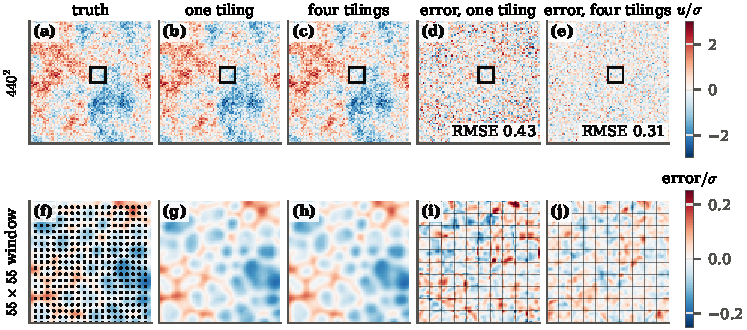
\includegraphics{figures/fig11_da_snapshot.pdf}
\caption{One steady-state analysis at $330^2$ ($\dlat=21\,600$, 64 members,
cycle 78 of 100), fields divided by the training standard deviation.
Top: the whole domain; the square marks the $55\times55$ window shown
below. (a, e) Truth, with the observation sites in the window; (b, f)
free run, the mean of the 64 unassimilated members, which have
decorrelated from the truth and from each other, so their mean keeps
only the large-scale pattern; (c, g) analysis, the decoded ensemble
mean; (d, h) analysis error, with patch edges drawn in the window.
Root-mean-square errors in field units. The analysis recovers the
cellular pattern everywhere; much of its residual error is small-scale
and largest at patch edges.}
\label{fig:da_snapshot}
\end{figure*}

\begin{figure*}[htbp]
\centering
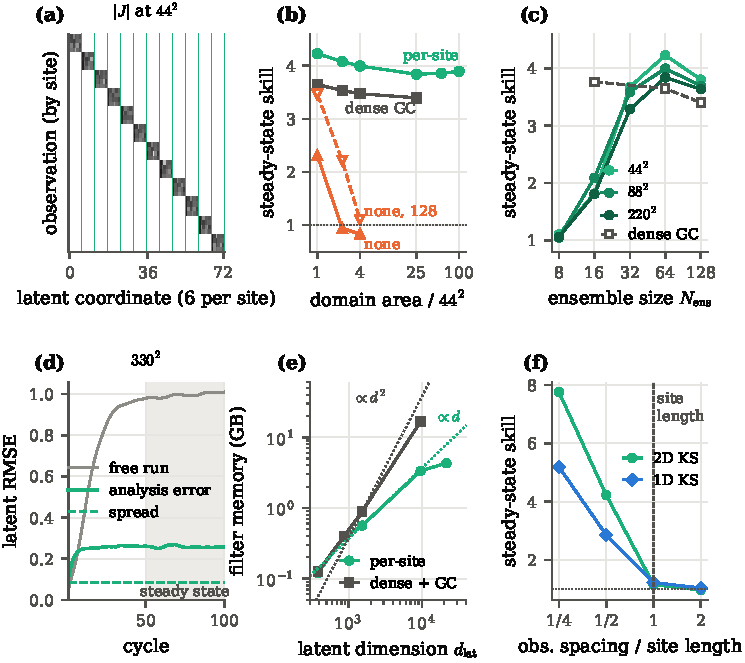
\includegraphics{figures/fig09_2d_da.pdf}
\caption{Data assimilation in the 2D KS latent field. (a) Magnitude of
the observation Jacobian at $44^2$, computed densely by reverse-mode
differentiation, with observations sorted by the site that owns them
(12 of the 64 sites): it is exactly zero outside the six columns of each
site (largest off-block entry $0$, largest entry $1.6$), as
Proposition~\ref{prop:blockdiag} states. (b) Steady-state skill against
domain area with 64 members (and 128 for the unlocalized filter): the
per-site filter keeps its skill over a hundredfold area; the
unlocalized filter fails where the truth's $n_+$ ($42$--$44$ at $44^2$,
$93$--$101$ at $66^2$) exceeds the ensemble. (c) Skill against ensemble size
for the per-site filter at three sizes, and for the dense filter with
Gaspari--Cohn localization at $44^2$. (d) Per-cycle analysis error,
spread and free-run error at $330^2$ ($\dlat=21\,600$); shaded: the
steady-state window. (e) Peak memory of the filter alone against latent
dimension, with guides proportional to $\dlat$ and $\dlat^2$ through the
$88^2$ points; from $220^2$ to $330^2$ the per-site filter's memory grows less
than linearly. (f) Skill against observation spacing in units of the
site length, for 2D KS at $44^2$ and 1D KS at $L=200$: assimilation fails once the spacing
reaches the site length in both systems.}
\label{fig:da_2d}
\end{figure*}

\begin{table*}[htbp]
\caption{2D KS data assimilation across domain sizes, steady-state
skill (calibration in parentheses), observation spacing $2.75$, 100
cycles. $n_+$: positive Lyapunov exponents of the truth; $^a$of the
transferred model, no truth at this size. Per-site: the per-site filter
with 64 members, seed 0 and, after the comma, seed 1. Dense GC: dense
filter with Gaspari--Cohn localization, 64 members. Unlocalized: dense
filter without localization, 64 and 128 members. ---: not run (the dense
filter's memory grows with the square of the area).}
\label{tab:da_2d_sizes}
\widetabular{lcccccc}{
size & $\dlat$ & $n_+$ & per-site, 64 & dense GC, 64 & unlocalized, 64 & unlocalized, 128 \\
\hline
\tabinput{tables/tab07_2d_sizes}}
\end{table*}

\begin{table*}[htbp]
\caption{Steady-state skill against ensemble size, 2D KS. Per-site
filter (perturbed observations) at four domain sizes; its deterministic
transform variant at $44^2$; dense filter with Gaspari--Cohn localization
at three sizes. ---: not run.}
\label{tab:da_2d_ensemble}
\widetabular{ccccccccc}{
$\Nens$ & per-site $44^2$ & $66^2$ & $88^2$ & $220^2$ & transform $44^2$ & dense GC $44^2$ & $66^2$ & $88^2$ \\
\hline
\tabinput{tables/tab07_2d_ensemble}}
\end{table*}

%----------------------------------------------------------------------
\subsection{Observation density and the one-dimensional results}
\label{sec:da_1d}
%----------------------------------------------------------------------

\para{How dense the network must be.} In both systems the filter needs
observations inside every patch. With the per-site filter at $44^2$ and
$\Nens=64$, the steady-state skill is $7.8$ at an observation spacing of
$1.4$ length units, $4.2$ at $2.75$, and $1.2$ and $1.0$ at $5.5$ and $11$. In
1D at $L=200$ with the particle flow filter and Gaspari--Cohn
localization it is $5.2$, $2.9$, $1.2$ and $1.0$ at spacings $1.6$, $3.1$,
$6.25$ and $12.5$. Assimilation fails once the spacing reaches the site
length ($5.5$ in 2D, $6.25$ in 1D), well below the pattern wavelength
$2\sqrt2\,\pi\approx8.9$: a site whose patch holds no observation is
corrected only through its neighbours' covariances, which the latent
field carries poorly. All other runs use half the site length.

\para{1D after transfer.} Table~\ref{tab:da_1d} and Fig.~\ref{fig:da_1d} give the 1D results at
$L=200$ and $400$, two and four times the training size, at a fixed
observation spacing of $3.125$. With localization, skill is $2.3$--$3.0$ for
every ensemble of 16 or more members, at both sizes and with both
filters. Without localization the filter makes the estimate worse than
no assimilation (skill below 1) until the ensemble is large enough, and
how large depends on the domain: at $L=200$, where $n_+=26$--$27$, it is marginal
at 64 members ($1.1$--$1.3$) and works at 128 ($2.5$--$2.7$); at $L=400$, where
$n_+=50$--$51$, it fails at 64 ($0.8$), is marginal at 128 ($1.2$--$1.4$) and
works only at 256 ($2.5$--$2.7$). The number of members an unlocalized
filter needs doubles with the domain, as the bound of
Sec.~\ref{sec:da_setting} predicts, while the localized filter needs
the same 16 at both sizes. The particle flow filter and the ensemble
Kalman filter differ by at most $0.4$ in skill and show the same pattern
at every point, so the result does not depend on the analysis scheme.

An earlier version of this experiment scaled the observation stride
with the domain, which doubled the observation spacing with every
doubling of $L$, to $6.25$ at $L=200$ and $12.5$ at $L=400$. At those spacings
the localized filter's skill at $L=200$ was about $1.3$, against $2.9$ at
the fixed spacing used here.

\para{Distance-free localization.} Sampling error correction
\citep{anderson2012} needs no distance, and is therefore the natural
competitor of a latent field that has one. At the training size, in an
earlier comparison with 40 cycles, SEC applied to a global latent vector
beat Gaspari--Cohn applied to the local field at every ensemble size,
with analysis errors $5$--$25\%$ lower. That comparison confounds the
localization with the architecture (two different autoencoders), and at
$L=100$ the taper is non-zero on 11 of the 16 sites of the ring, so it
hardly localizes. At the transfer size the comparison can be made
on one latent. The SEC-corrected covariance, formed elementwise, is
indefinite at five of six ensemble sizes, and the particle flow filter,
which factorizes it, fails. This is a property of the matrix form, not of
SEC: projecting the corrected matrix onto the positive semidefinite cone,
or applying the correction to each regression coefficient in a serial
filter, the form \citet{anderson2012} uses, both run at every ensemble
size. Gaspari--Cohn beats both at every size below 256 members: by a
factor of up to $1.7$ against the projected form (both with the particle
flow filter) and up to $3.5$ against the serial form (both ensemble
Kalman filters), and the serial form does not help at all below 128
members (Table~\ref{tab:da_1d}). SEC removes
sampling noise from correlations; a distance taper also removes the many
weak true correlations between distant sites, and that is what the small
ensemble cannot afford to estimate.

\begin{figure*}[htbp]
\centering
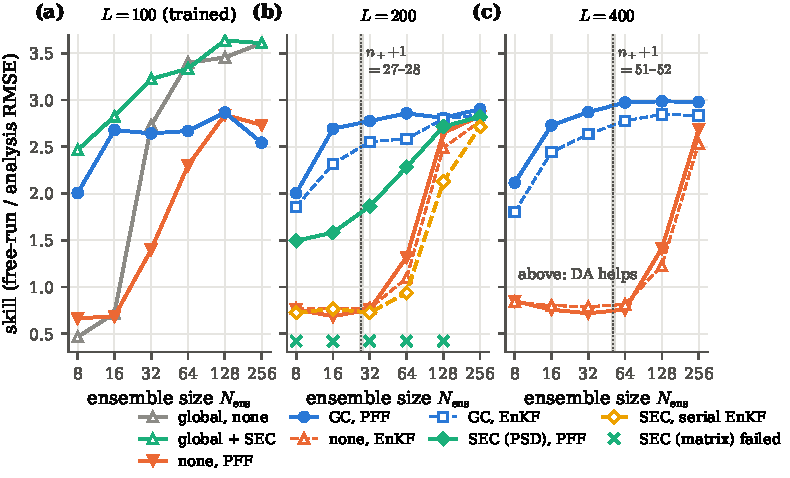
\includegraphics{figures/fig08_1d_da.pdf}
\caption{1D KS data assimilation: skill (free-run error over analysis
error; above the dotted line assimilation helps) against ensemble size,
observation spacing $3.125$ in every panel. (a) Training size $L=100$
(earlier sweeps, 40 cycles, whole-run skill): a global latent vector
without localization and with sampling error correction (SEC), and the
local field without localization and with Gaspari--Cohn (GC), particle
flow filter, drawn with the symbols of the particle-flow curves in (b,c). (b) $L=200$ and (c) $L=400$, the local model transferred
without retraining (100 cycles, steady state): no localization and GC,
for the particle flow filter (solid) and the ensemble Kalman filter
(dashed); in (b) also SEC after projection onto the PSD cone and in a
serial filter, with crosses at the ensemble sizes where SEC in matrix
form failed. The shaded line marks $n_++1$ for the truth. With
localization a 16-member ensemble suffices at both sizes; without it,
the ensemble must exceed the number of unstable directions by a margin,
and that number doubles with the domain.}
\label{fig:da_1d}
\end{figure*}

\begin{table*}[htbp]
\caption{1D KS data assimilation after transfer: steady-state skill
(free-run error over analysis error, cycles 51--100) at a fixed
observation spacing of $3.125$, model trained at $L=100$. Pairs: no
localization / Gaspari--Cohn (half-width 3 sites). Last two columns
($L=200$ only): sampling error correction with the particle flow filter
after projection onto the PSD cone, and in a serial ensemble Kalman
filter. Skill below 1 means the filter is worse than no assimilation.}
\label{tab:da_1d}
\widetabular{ccccccc}{
$\Nens$ & PFF, $L=200$ & PFF, $L=400$ & EnKF, $L=200$ & EnKF, $L=400$ & SEC-PSD & serial SEC \\
\hline
\tabinput{tables/tab07_1d_da}}
\end{table*}
%----------------------------------------------------------------------
\subsection{Cost and memory}
\label{sec:da_cost}
%----------------------------------------------------------------------

Table~\ref{tab:da_cost} gives what the filters cost. Memory is the peak
resident memory of the filter alone, measured as the peak over a run
minus the peak once the truth has been generated. The per-site filter
needs $0.12$, $0.39$, $0.56$, $3.35$ and $4.30$~GB at $\dlat=384$, $864$, $1536$,
$9600$ and $21\,600$. From $88^2$ to $220^2$ the latent dimension grows
$6.25$-fold and the memory $5.96$-fold, and from $220^2$ to $330^2$ the
dimension grows $2.25$-fold and the memory $1.28$-fold: the filter's memory
grows no faster than the domain area, as Proposition~\ref{prop:blockdiag}
implies. The dense filter needs the
same at the native size but $16.75$~GB at $220^2$, about 24 copies of one
$\dlat\times\dlat$ matrix; at $330^2$ a single such matrix is $3.5$~GB and at
$440^2$ it is $11$~GB, so we did not run it there.

Time is less favourable to the per-site filter at small sizes. Over a
whole run, including the integration of the PDE truth, the per-site
filter takes two to four times the dense filter's CPU time up to $88^2$,
because it loops over sites in Python while the dense filter performs a
few large matrix products. The two cross between $88^2$ and $220^2$
($1450$ against $1914$~s at $220^2$), and from there the per-site filter's
time grows in proportion to the area ($\times4.4$ from $220^2$ to $440^2$
for $\times4$ in area). The deterministic variant is about $40\%$ faster
than the perturbed-observation one, having no observation draws. The
CPU times carry run-to-run noise of tens of percent from other jobs on
the same machine (the $66^2$ point is slower than the $88^2$ one); we
have not profiled the per-site loop, which is the obvious target for a
vectorized implementation. The observation Jacobian itself is cheap:
its six forward passes take $1.3$~ms at $44^2$ and $49$~ms at $440^2$, where
dense reverse mode would need one pass per observation
(Appendix~\ref{app:da_jacobian}).

\begin{table}[htbp]
\caption{Cost of the per-site and dense filters, 2D KS, $\Nens=64$, 100
cycles. $\dlat$: latent dimension; filter memory: peak resident memory
minus the peak after the truth is generated (GB); $\dlat^2$: memory of one
dense $\dlat\times\dlat$ matrix in double precision (GB); CPU: whole-run
user plus system time, including the PDE truth (s). ---: not run, or no
clean memory measurement yet.}
\label{tab:da_cost}
\begin{ruledtabular}
\begin{tabular}{lcccccc}
size & $\dlat$ & \multicolumn{2}{c}{filter memory} & $\dlat^2$ & \multicolumn{2}{c}{CPU} \\
 & & per-site & dense & & per-site & dense \\
\hline
\tabinput{tables/tab_da_cost}
\end{tabular}
\end{ruledtabular}
\end{table}
